% ch05-consistency-vs-validation.tex — Consistency vs Validation 2×2 Matrix
% Shows the four quadrants with labels and brief examples.
% Pedagogical purpose: make the independence of the two axes visually clear.
\documentclass[tikz,border=5pt]{standalone}
\usepackage{fontspec}
\setmainfont{Times New Roman}
\usepackage{unicode-math}
\setmathfont{Cambria Math}
\usetikzlibrary{shapes.geometric,shapes.misc,positioning,fit,backgrounds,arrows.meta,matrix}

\begin{document}
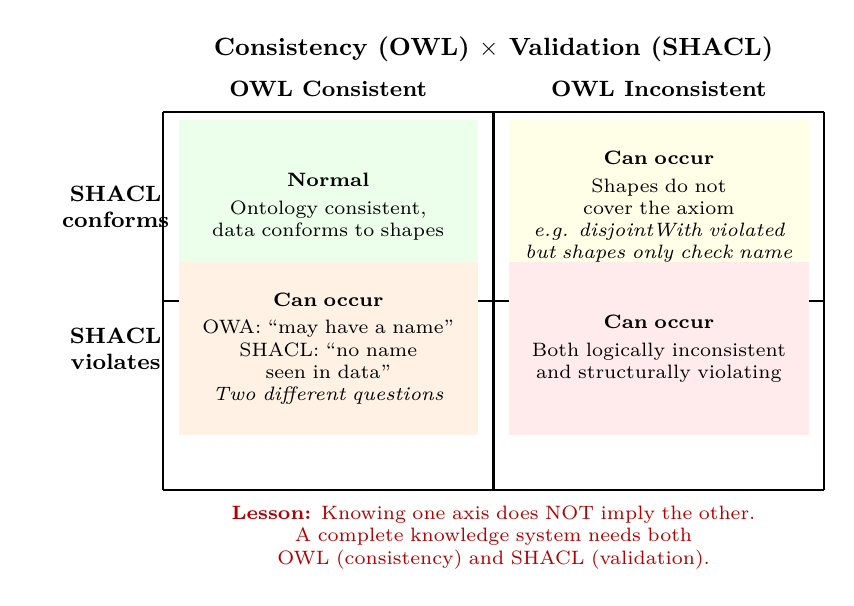
\begin{tikzpicture}[
  cell/.style={minimum width=3.8cm,minimum height=2.2cm,align=center,
               font=\scriptsize,inner sep=4pt,text width=3.5cm},
  header/.style={font=\footnotesize\bfseries,align=center},
  axislabel/.style={font=\small\bfseries},
]

% Title
\node[font=\small\bfseries] at (0,3.8) {Consistency (OWL) $\times$ Validation (SHACL)};

% Matrix grid
\draw[thick] (-4.2,3.0) -- (4.2,3.0);
\draw[thick] (-4.2,0.6) -- (4.2,0.6);
\draw[thick] (-4.2,-1.8) -- (4.2,-1.8);
\draw[thick] (-4.2,3.0) -- (-4.2,-1.8);
\draw[thick] (0,3.0) -- (0,-1.8);
\draw[thick] (4.2,3.0) -- (4.2,-1.8);

% Column headers
\node[header] at (-2.1,3.3) {OWL Consistent};
\node[header] at (2.1,3.3) {OWL Inconsistent};

% Row headers
\node[header,text width=2cm] at (-4.8,1.8) {SHACL\\conforms};
\node[header,text width=2cm] at (-4.8,0.0) {SHACL\\violates};

% Cell A: consistent + conforms (normal)
\node[cell,fill=green!8] at (-2.1,1.8)
  {\textbf{Normal}\\[2pt]
   Ontology consistent,\\data conforms to shapes};

% Cell B: inconsistent + conforms (possible!)
\node[cell,fill=yellow!10] at (2.1,1.8)
  {\textbf{Can occur}\\[2pt]
   Shapes do not cover the axiom\\
   \textit{e.g. disjointWith violated\\but shapes only check name}};

% Cell C: consistent + violates (OWA vs data-check)
\node[cell,fill=orange!10] at (-2.1,0.0)
  {\textbf{Can occur}\\[2pt]
   OWA: ``may have a name''\\
   SHACL: ``no name seen in data''\\
   \textit{Two different questions}};

% Cell D: inconsistent + violates
\node[cell,fill=red!8] at (2.1,0.0)
  {\textbf{Can occur}\\[2pt]
   Both logically inconsistent\\and structurally violating};

% Key insight
\node[font=\scriptsize,text=red!70!black,align=center,text width=8cm] at (0,-2.4)
  {\textbf{Lesson:} Knowing one axis does NOT imply the other.\\
   A complete knowledge system needs both OWL (consistency) and SHACL (validation).};

\end{tikzpicture}
\end{document}
